\documentclass[12pt]{article}
\usepackage{hyperref}
\usepackage{gensymb}
\usepackage{imakeidx}
\usepackage{amsmath}
\usepackage{listings}
\usepackage{graphicx}
\usepackage{sidecap}
\usepackage{pgfplots}
\graphicspath{ {./Images/} }

\makeindex

\begin{document}
\title{Modelling Low Earth Orbit Constellations for Networking}
\author{Joseph McGuchan}
\maketitle
\thispagestyle{empty}

%TODO Cover Sheet

\newpage

%TODO Declaration of Originality

I, Joseph Law McGuchan of King's College, being a candidate for Part II of the Computer Science Tripos, hereby declare that this dissertation and the work described in it are my own work, unaided except as may be specified below, and that the dissertation does not contain material that has already been used to any substantial extent for a comparable purpose.

Signed %TODO

Date %TODO

\newpage

%TODO Proforma

%Your candidate number.
%The Title of your Project. 
Modelling Low Earth Orbit Constellations for Networking
%The Examination and Year.
%Word-count for the dissertation.
%Final line count: Number of lines written by the *student* in the final version of their %software work.
%Project Originator.
%Project Supervisor.
%At most 100 words describing the original aims of the project.
%At most 100 words summarising the work completed.
%At most 100 words describing any special difficulties that you faced. 
%(In most cases the special difficulties entry will say “None”.)

\newpage

\tableofcontents

%==============================================================================================================================
%----------------------------------------------------------------------------------------------------------INTRODUCTION-------------------------------------------------------------------------------------------------------
%==============================================================================================================================
\section{Introduction}

SpaceX are planning to launch a constellation of 4,425 low Earth orbit communication satellites in the next few years. The objective of this constellation, called Starlink, is to provide low-latency internet connection across the world.

The satellites in this network will be in constant motion, not just relative to the ground, but relative to one another, creating a network with a constantly changing topology and associated latencies. The question of how to structure such a network, and what the resultant latencies of said network will be, has not been thoroughly explored, but it will become increasingly relevant as more and more companies build similar constellations. If these Constellations prove to provide significant gains in latency while providing competitive bandwidth, they might render previous submarine optical cables obsolete.

My goals are:
\begin{enumerate}
	\item To create visualizations of the SpaceX constellation.
	\item To experiment with different topologies of the SpaceX network and test their associated latencies. 
\end{enumerate}

%============================================WHAT IS STARLINK======================================================
\subsection{What is Starlink?}

The purpose of Starlink is to provide low latency internet connections, as of 21/11/18, there are two companies offering satellite internet services, Excede\cite{ExcedeWebsite}, and Hughes, whose 9202 BGAN Land Portable Satellite Terminal offers connection speeds up to 464kbps\cite{HughesWebsite}. These companies largely target domestic use in rural areas which don’t have a faster coverage, and corporations, providing internet connections to airplanes and cargo ships. Currently, Satellite Internet connection is a last resort, something turned to when conventional means of connection are not available, Starlink intends to invert this, turning satellite internet into the premium option. 

The difference between Starlink and currently existing brands is that current brands use geostationary satellites \cite{HughesPressRelease}, while Starlink will use LEO satellites. The significantly shorter distance will create much shorter paths for signals. On top of this, SpaceX will be utilizing laser communication between satellites, as opposed to the competitors who have little to no intra-satellite communication. In the vacuum of space, lights travels 47\% faster than in glass \cite{PropertiesOfGlass}. Therefore, in theory, a LEO network utilising lasers would achieve latencies far lower than that by even the best terrestrial fiber optic connections over long distances.

%============================================WHY FOCUS ON STARLINK======================================================
\subsection{Why Focus on Starlink?}

Starlink is only one of a number of different LEO internet networks that have been proposed, so why should I focus on it's topology? Ideally, I would like the conclusions of my study to be generalized to many other LEO constellations. However, constellations are approved by the FCC on a case-by-case basis, using a complicated and changing system of legislation, it's not easy to know what a normal network looks like. By analyzing the properties of a network of my own design, I run a much greater risk of coming to conclusions that cannot be generalized, as I am not working on an FCC-approved constellation.

What about the constellations of other companies? %TODO WHEN GOVERNMENT FUNDING RETURNS

By analyzing the properties of Starlink, we are analyzing a network that is confirmed legally and scientifically plausible.

But there is another reason to investigate Starlink. As the largest of most high-profile attempts to build a LEO internet backbone, Starlink represents themost significant competitor to other emerging sattelite communications networks and the one more likely to become dominant in future years. By theorising about it's properties now, we can prepare ourselves for the changes Starlink might pose to communications in the upcoming years.

%============================================WHY CREATE A VISUALISATION======================================================
\subsection{Why Create a Visualisation?}
When it comes to understanding a network such as starlink, a visual description is incredibly valuable. By visualizing the network we can develop an intuition for how it operates, and use that intuition to develop ideas for new algorithms and structures for testing.

Creating a visualization also poses a minimal additional cost on my part, as to accurately model the latencies between base stations I will need to simulate satellite positions and links anyway.

%============================================MARK HANDLEY'S WORK======================================================
\subsection{Mark Handley's Work}

%TODO

My initial proposal for the project was inspired by the findings of an existing study done  by Mark Handley, since proposing the project, Mark Handley has made his results publicly available\cite{OriginalReport}, so my new goal will be to replicate and expand upon his findings.

%============================================WHAT I WILL BE USING======================================================
\subsection{What I Will Be Using}
To create the visualization I will be using the open-source game engine Godot. Using a game engine struck me as the simplest way to create a visualization tool, and Godot, being powerful, open-source, and capable of running easily on many devices, seemed like the ideal choice.

For the parts of code related to visualization I will be using godot's build in script GDScript, which is easy to use and specifically designed to integrate well with the godot engine. For parts of the code related to simulation I will use C\#, which godot is compatible with, and which offers significance performance improvements over gdscript.

%==============================================================================================================================
%----------------------------------------------------------------------------------------------------------PREPARATION---------------------------------------------------------------------------------------------------------
%==============================================================================================================================
\section{Preparation}


%============================================STARING POINT======================================================
\subsection{Starting Point}

Most of the information I will be using for the structure of the SpaceX network comes from their application to the FCC on March 29th, 2018\cite{FCCApplication}, and their technical attachment\cite{TechnicalAttachment}, which outlines the various orbital spheres, planes within each sphere, and various other details of the constellation. I will also be building on insights gleaned from Handley's original research. The insights that I will be building off of are:


%TODO

SpaceX have already sent up two test sattelites, and according the Elon Musk, they are working very well, providing a latency of only 25ms\cite{ElonMuskTweet}.

%TODO

%============================================THE STRUCTURE OF STARLINK======================================================
\subsection{The Structure of Starlink}

There is a lot we do not know about Starlink, but this is what we can infer from SpaceX’s application to the FCC\cite{FCCApplication}, 

Starlink is a constellation of 4,425 LEO sattelites with a further proposed. %TODO when govern funding back

We will be examining only the 4,425 sattelites proposed for the first implemantation of Starlink, as these intend to provide a viable network by temselves, and additional sattelites might overwhelm my visualisation techniques. 

\begin{figure}
\begin{center}
\label{fig:Starlink Orbits}
\caption{The layout of Starlink}
\begin{tabular}{|c|c|c|c|c|c|}
\hline
\multicolumn{6}{|c|}{SPACEX SYSTEM CONSTELLATION} \\
\hline
Parameter & Initial Deployment & \multicolumn{4}{|c|}{Final Deployment} \\
& (1,600 satellites) & \multicolumn{4}{|c|}{(2,825 satellites)} \\
\hline
Orbital Planes & 32 & 32 & 8 & 5 & 6 \\
Sattelites per Plane & 50 & 50 & 50 & 75 & 75 \\
Altitude & 1150km & 1110km & 1130km & 1275km & 1325km \\
Inclination & 53\degree & 53.8\degree & 74\degree & 80\degree & 70\degree \\
\hline
\end{tabular}
\end{center}
\end{figure}

In it's application to the FCC SpaceX was required to state any notable debris that might not burn up if a satellite were to descend from orbit. Among the components listed where 5 silicon carbide “communication components”, silicon carbide is used in mirrors for laser communication links, and we can therefore conclude that SpaceX's satellites will have, at most, 5 available links to form with nearby satellites.

We also know information about how Starlink satellites will communicate with ground stations, a base station may only connect with a satellite at an inclination less than 40\degree from the vertical using Radio Frequency (not laser) connections. Connections will be stronger to satellites directly overhead, however as Starlink does not provide much information in exactly how their intra-satellite communications work, speculations on bandwidth will not prove to be helpful.

%============================================MODELLING SATELLITES IN ORBIT======================================================
\subsection{Modelling Sattelites in Orbit}

Typically, an orbit around the surface of the earth is described by:

\begin{description}
\item[Distance Above the Surface]
\item[Inclination]
This is the angle between the orbital plane, and the equatorial plane, (the plane on which the equator lies).
\item[Longditudonal Offset]
If inclination is greater than 0\degree, then the orbital plane and equatorial plane will intersect at a line, the angle between this line and the plane described by the great circle at longditute 0\degree is the longditudonal offset. In other words, the Longditudonal offset is the Londitudute of the point where this line passes through the surface of the earth.
\item[Eccentricity]
The eccentricity coefficient describes the “squashness” of the orbit. For the time being, we will be ignoring this...
\item[Retrograde]
A retrograde orbit is one that goes against the rotation of the earth, typically these are described by orbits with a longditudonal offset greater than 180\degree. It is significantly more expensive to put a sattelite into a retrograte orbit, and is essentially never done.
\end{description}

Furthermore, an individual satellite's position in an orbit can be described by:

\begin{description}
\item[True Anomaly]
The angle between the line drawn from the origin to the satellite, and the line drawn from the origin to the point on the sattelite's orbit of longditude 0.
\item[Phase Offset]
This is the satellite's true anomaly at time 0.
\end{description}

In our model, true anomaly is the only variable that changes. The way it changes is uniquely determined by the other 6 variables. The rate of change of true anomaly, the anglular velocity, is given by

\[\sqrt{\frac{GM}{r^3}}\]

Where r is the distance from the origin, or altitude + radius of the Earth.

Note that while altitude is constant (eccentricity = 0) velocity is unchanging, and true anomaly can be described as a linear function of time.

The position of a satellite is calculated by taking it’s true anomaly and adding it’s angular velocity multiplied by the timestep (real timesince last frame update * some factor). The location is then calculated through a series of transformations performed on the true anomaly:

\begin{enumerate}
\item We take a vector (r, 0, 0) where r is the distance above the surface + the radius of Earth.
\item We rotate this point around (0, 1, 0) (the line through the poles) by the true anomaly.
\item We rotate this point around (1, 0, 0) (the line from 0 longitude to 180 longitude through the equator) by the inclination.
\item We rotate this point around (0, 1, 0) again by the longitudinal offset.
\end{enumerate}

Because the only variable that is changed is the true anomaly, and the x, y, and z coordinates are determined by only this variable and a series of fixed variables, we do not run the same risks normal discrete physics models face when describing continuous behavior, such as the energy of the system changing, or orbital precession (the point of furthest distance moving steadily), as we will not be approximating a continuous process from a series of discrete steps but instead will be taking samples from a continuous function.

For the rest of this document, a satellite will be denoted by $x_{i,j,k}$. Describing the kth satellite on the jth orbital place in the ith orbital sphere. $L$ gives the number of orbital spheres, with $M_i$ giving the number of orbits in orbital sphere i, and $N_i,j$ giving the number of satellites in the jith orbit of the ith sphere.

%===================================================UNKOWN VARIABLES========================================================
\subsection{Unkown Variables}
While we can learn a lot from SpaceX's applications, there are still a number of variables that are left undetermined. 

\begin{description}	
\item[Phase Offset]
As we do not know for certain how satellites will be positioned in orbits, we also do not know how they will be positioned relative to other orbits. The phase offset of an obit $o_{i,j}$, $po_{i,j}$, can be described as a number from 0 to 1, where, $\forall k$, 0 indicates that  $x_{i,j,k}$ will cross the equator at the same time as $x_{i,j+1,k}$, and 1 indicates that satellite $x_{i,j,k}$ will cross the equator at the same time as $x_{i,j+1,k+1}$. This number will have to be some fraction of the total number of orbits, to guarantee that the first and last orbits are properly aligned.

\item[Sphere Offset]
As well as satellites being offset from one another, whole spheres can be offset too. I will only be looking at a single sphere in my study, however, so this variable will not be examined.

\item[Link usage]
Each satellite will have a maximum of 4 links, however, we do not as of yet know which arrangements of links are the most optimal.

In his study Mark Handley uses two links to connect $x_{i,j,k}$ to $x_{i,j,k+1}$ and $x_{i,j,k-1}$. He then uses the other two to connect $x_{i,j,k}$ to $x_{i,j+1,k+h_i}$ and $x_{i,j-1,k-h_i}$, where $h_i$ is a variable that describes how "diagonal" these sideways links should be. For $j = 0$ and $j = number_of_orbits$, $x_i,0,k$ connects to $x_i$, %TODO

In general, a fixed-link linking method can be described by an n/2 by 2 matrix, where n is the number of links each satellite has free. In this case, that means a 2x2 matrix.
\end{description}

%==============================================================================================================================
%----------------------------------------------------------------------------------------------------------IMPLEMENTATION----------------------------------------------------------------------------------------------------
%==============================================================================================================================
\section{Implementation}

%============================================REPOSITORY OVERVIEW======================================================
\subsection{Repository Overview}

%============================================CODING FOR VISUALISATION AND EFFICENT ALGORITHMS======================================================
\subsection{Coding for Visualisation and Efficent Algorithms}

This implementation chapter is devideed into two main sections, the first section will go over how I represented the constellations and the code I wrote to perform tests on this model, the second section will go over the executable file, it's structure, and how to use it. While these sections are seperate in my report, they were developed concurrently, and are connected to each other.  As I visualised the constellation, I was able to gain a better understanding of it's structure, this directed the properties of the network I wanted to examine, which in turn effected the tests I wanted to create and so the algorithms I needed to implement. Furthermore as Godot is designed to model 3d environments it provides a number of functions that in turn influenced how I wrote my algorithms, most rotably Godot provides a simple framework for multithreading through a \lstinline{_process} funtion that any calss extending Node can override and which is called on every step by the engine. Godot handles multithreading of the process function internally. This gave me the opportunity to exploit threading to improve the efficency of the program without having to do any extra work. All that said, I think to is clearer to divide these two halves of the program when talking about my implementation.

After these two sections will be one more outlining observations that were made of the network's behaviour during my experimenting on it, and how these observations lead to further development in my linking algorithms.

%============================================CODING FOR VISUALISATION AND EFFICENT ALGORITHMS======================================================
\subsection{Modelling the Network}

%-----------------------------------------------------------------------------DIFFICULTIES OF MODELLING ORBITS-----------------------------------------------------------------------------
\subsubsection{Difficulties of Modeling Orbits}
On Implementation, I found that my planned method of implementing orbits was flawed, being able to simulate only 500 satellites in motion before slowing down. Because of this, I changed to a precomputed method. In this method, orbits are precomputed as a number of transformations, and the position of satellites is calculated by interpolating adjacent transformations, this sacrifices some accuracy, but vastly increases the computation speed. It is important that orbits be described by transformations (a combination of a point and rotation) so that satellites can be oriented to ways have the earth below them from their reference frame. This makes a umber of computations later on easier.

%-----------------------------------------------------------------------------REPRESENTING LINKS-----------------------------------------------------------------------------
\subsubsection{Representing Links}
There are 3 primary ways to represent a graph for algorithms:

\begin{description}
\item[Adjacency Matrix] An NxN matrix of values representing all possible connections. Obviously inefficient for a sparse set of connections like this.
\item[Adjacency List] Associate each Satellite with a list of the vertices it is connected to. Space efficient, but creates difficulty in running Dijkstra's algorithm.
\item[Edge List] Create a list of edges that refer to vertices. This is useful for algorithms that require iterating through all edges like Dijkstra's algorithm. But to find the adjacent satellites to any given satellite requires searching through the whole list.
\end{description}

Initially, I used adjacency lists, this lead to a number of problems.

\begin{itemize}
\item Some algorithms require a list of all edges, which is very hard to obtain with adjacency lists.
\item When drawing edges in the visualization, each would be drawn twice, for each vertex they were associated with.
\item When updating links, values such as the distance between two verticies had to be computed twice for each vertex.
\end{itemize}

Instead I created a new class of objects representing links, and gave each vertex a reference to the links associated with it. 

In Godot, all drawn objects require one "parent" (different to class inheritance) which is already a drawn object. Children inherit the position and rotation of their parents, and rotating a group of objects is significantly more efficient than rotating a single object alone. Because of this, backwards and forward links, which do not change distance or position relative to the satellite, should be made children of the satellite, and they will then never have to be updated. Because of this, all links have a primary and secondary satellite. Which the link always being the child of the primary satellite.

%-----------------------------------------------------------------------------PATTERNS USED-----------------------------------------------------------------------------
\subsubsection{Patterns used}

Due to the extensive combustibility of the network, I elected to use the Template Method pattern in three separate locations.

\begin{itemize}
\item To describe different linking methods.
\item To describe various different ways of colorizing the network to highlight certain properties.
\item To describe various tests to be applied to the network.
\end{itemize}

I also utilized a variant of the Builder pattern for describing constellations and tests. The ConstellationDescription class is initialized with a description of a constellation similar to what was given above, including the tests and colouring method I want to use on the class. This allowed me to easily categorize and load new constellations.

%-----------------------------------------------------------------------------DIJKSTRA'S ALGORITHM-----------------------------------------------------------------------------
\subsubsection{Dijkstra's Algorithm}

I used Dijkstra's algorithm in order to calculate shortest paths around the network, with the modification to allow for quickly retrieving the shortest path when used. Somewhat surprisingly, C sharp doesn't come with a priority queue, so I used one from \url{https://visualstudiomagazine.com/Articles/2012/11/01/Priority-Queues-with-C.aspx?Page=2}. And used comparisons from \url{https://github.com/BlueRaja/High-Speed-Priority-Queue-for-C-Sharp}.

%-----------------------------------------------------------------------------CALCULATING LATENCY ACROSS PATH-----------------------------------------------------------------------------
\subsubsection{Calculating the Latency Across a Path}

There are 4 factors that effect the latency of a path, some of which are easy to model, and others are significantly more tricky.

\begin{description}
\item[Processing delay] The time it takes router to process the packet header, this is typically insignificant and will bee assumed to be 0.
\item[Queuing delay]  The time the packet spends in routing queues, this is dependant on the load on the network and is therefore not easy to predict. I will be calculating lanency assuming the best case scenario, which is no queing delay.
\item[Transmission delay] The time it takes to push the packet onto the link. This is of course dependant on the size of the packet, but for the smallest packet sizes this value is negligable. 
\item[Propagation delay] The time the signal spends in transmission, since all connections are of the form of electromagnetic waves this is simply the path length divided by the speed of light.
\end{description}

Because of this, the only calculation needed to calculate needed to get the latency of a path is to divide it's length by the speed of light in a vaccum. To calculate the round trip time (RTT), which is typically used when advertising linking systems, we simply multiply this value by two.


%-----------------------------------------------------------------------------REPRESENTING A CONSTELLATION-----------------------------------------------------------------------------
\subsubsection{Representing a Constellation}
Constellations in my database are described in the a simple format that allows for much portability, this figure contains how to describe one theory or how the spaceX constellation might be arranged.

\begin{figure}
\label{fig:Starlink Within Program}
\caption{An example for how a constellation might be described.}
\begin{center}
\begin{tabular}{ | c | c  | c | c | c | c | }
	\hline
	Number of Orbital Spheres & \multicolumn{5}{| c |}{5} \\
	\hline
	\hline
	Sphere Number & 1 & 2 & 3 & 4 & 5\\ 
	\hline
	Altuitude & 1150km & 1110km & 1130km & 1275km & 1325km \\
	Inlication & 53\degree & 53.8\degree & 74\degree & 80\degree & 7-\degree \\
	Number of Orbits & 32 & 32 & 8 & 5 & 6 \\
	Sattellites per Orbit & 50 & 50 & 50 & 75 & 75 \\
	Offset Between Orbits & & & & &\\
	Offset of Sphere & & & & &\\
	Linking Method & X & X & X & X & X \\
	\hline

\end{tabular}
\[
X = Handley(-1)
\]
\end{center}
\end{figure}

Notice the addition of offsets and linking methods, these are necessary to fully describe a constellation, but are not given in an FCC application.

%-----------------------------------------------------------------------------EFFICIENCY VS USABILITY-----------------------------------------------------------------------------
\subsubsection{Efficiency vs Usalibitly}
To do this requires the creation of numerous abstract classes and wrappers that would simplify more complex objects. There are two kinds of vertex, base stations and satellites, and two kinds of link, those between satellites and those between a satellite and base station. Each of these are children of general Vertex and Link classes, and it is these classes that are used by the various tests and algorithms that run on the netwrok. Initially my objective was to prioritise efficentcy at all costs, but as I continued to develop the code, it became necessary to implement redundancies and inefficent storing methods, like lists, in order to make the code more easily usable. I also created a generic Graph object that contained only a list of Verticies and a list of Links, and a VertexParth object that allowed for easy manipulation and testing of paths.

%============================================VISUALISATION======================================================
\subsection{Visualization}

For the earth texture I used a creative commons equirectangular map of the Earth. Equirectangular means that x and y values correspond to longditude and latitude. It was important that the map be equirectangular as this is the format that is compatible with being mapped to a sphere. \cite{Map}

%-----------------------------------------------------------------------------HOW TO USE THE EXE------------------------------------------------------------------------------------

\subsubsection{How to Use the Exe}

If you would like to see the program that was used to generate these images and results, simply download and run the exe hosted here %TODO

The exe will create files for test results in the same location as it is ran, as well as printing to the command line the results of tests as they are written.

It is reccomended that you run in Windows 10, as it is not garunteed to work in other operating systems.

You can navigate the simulation using the mouse, along with arrow keys or WASD. Press R to reset the whole simualtion. Use X and Z to move between different tests. Press ESC to toggle the mouse between captured (for moving the camera) and free.

All the tests run at 60x realtime, which I found to be a very good timefactor for observing overarching trends in the network.

\begin{figure}
\begin{center}
\label{fig:Keybindings}
\caption{Keybindings.}
\begin{tabular}{ | c | c  | }
	\hline
	Move Forward & W, Up Arrow \\
	Move Backward & S, Down Arrow\\
	Move Up & Q, Comma Key\\
	Move Down & E, Full Stop Key\\
	Move Left & A, Left Arrow \\
	Move Right & D, Right Arrow \\
	Restart Simualtion & R \\
	Toggle Free Mouse & Esc \\
	Next Test & X\\
	Previous Test & Z\\
	\hline
\end{tabular}
\end{center}
\end{figure}

There are a total of %TODO

%-----------------------------------------------------------------------------THE MOTION OF THE PLAYER------------------------------------------------------------------------------------
\subsubsection{The Motion of the Player}

One of the few pieces of code written in Godot's native language GDScript is the code that controls user interaction with software. It made sense to write this in GDScript as it is a much simpler language than C\#, and because a very simple tutorial of first person motion was available in GDScript\cite{FirstPersonMotion}. However this code required some adaptation to make it work in 3D, primarily the removal of a number of unnecessary features, and the addition of the ability to move up and down.

The code works using a "head" which is attached to a "neck". Left-right motions of the mouse are translated to left-right rotations of the neck, while up-down motions of the mouse are translated into up-down rotations of the head. keeping the head and neck separate mean that the player cannot turn themselves upside down. Motion is done relative to the head's view, with gentle smoothing applied to motion to give a more natural feeling.

%============================================INITIAL OBSERVATIONS OF THE NETWORK======================================================
\subsection{Initial Observations of the Network}

While working on the program I made a few notable obervations of the network. In this section I go through each of these observations and outline how it fed into what I was doing.

%-----------------------------------------------------------------------------THE STRUCTURE OF THE NETWORK------------------------------------------------------------------------------------
\subsubsection{The Structure of the Network}

One of the most notable observations of the network was it's unique, layered grid structure. To highlight this I applied a different hue to each orbit \ref{fig:Structure of Network}. As you can see, for a given point near the equator, there are in fact two very different kinds of Satellite moving overhead, those going North-East, and those going South-East. Towards the poles, on the other hand, all satellites are moving Eastward. This means that Satellites that pass very close to one another on the equator can end up on opposite sides of the Earth close to the poles. As described below, it is very likely that Satellites will only link to other satellites moving the same direction as them, and in my model I have reflected that. This means that for a given point on earth there will be two almost seperate grids moving overhead, one grid of satellites moving North-East, and another of satellites moving South-East.

\begin{figure}
\label{fig:Structure of Network}
\caption{The Starlink Constellation with a different hue appllied to each orbit.}
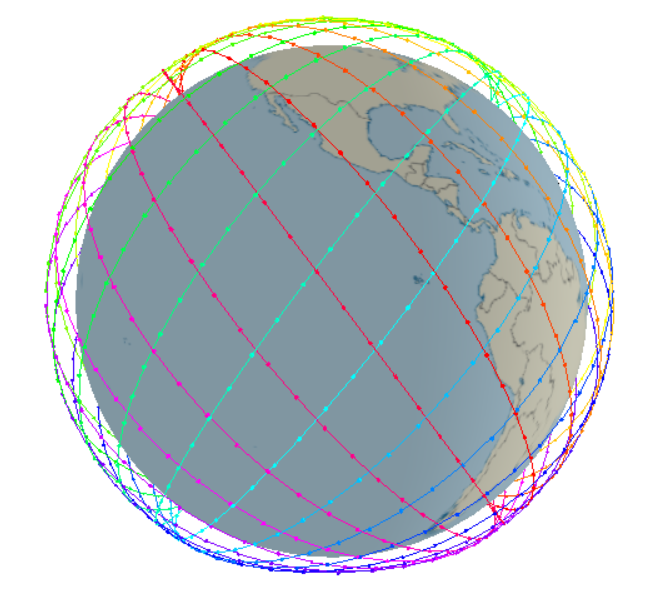
\includegraphics[width=0.3\textwidth]{Hue1}
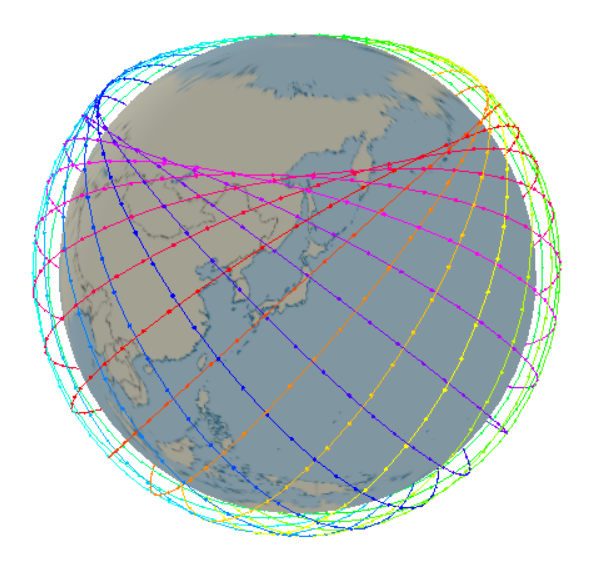
\includegraphics[width=0.3\textwidth]{Hue2}
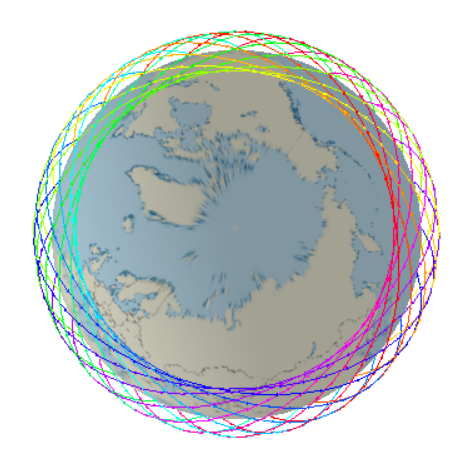
\includegraphics[width=0.3\textwidth]{Hue3}
\end{figure}


%-----------------------------------------------------------------------------THE MOVEMENT OF SATELLITES RELATIVE TO EACH OTHER------------------------------------------------------------------------------------
\subsubsection{Movement of Satellites Relative to Each Other}

I decided to track the path of a satellites neighbors relative to it and it's direction of movement over the course of an orbit around the Earth. In \ref{fig:Relative Paths of Satellites} the paths traced by nearby satellites is given. The satellites directly ahead of and behind a given satellite stay in a steady position relative to it and it's direction of motion, while those in adjacent orbits slowly figure eights. You can see in \ref{fig:The 9 Satellites Being Tracked} that there are other nearby satellites in different orbits, however these satellites are moving South while the highlighted satellites are moving North, meaning that they will be moving by far too quickly for the main satellite to track them as they pass. \cite{OriginalReport}

These results show that satellites in adjacent orbits will be moving in relatively slow and predicatable ways meaning it should be possible for a satellite to track a laser link to satellites in adgacent orbits. It also shows that links to satellites in the same orbit will be significantly easier as satellites in the same orbit maintain a constant position relative to one another.

\begin{SCfigure}
\centering
\label{fig:The 9 Satellites Being Tracked}
\caption{The 9 Satellites I tracked, the motion was logged relative to the position and direction of motion of the central satellite.}
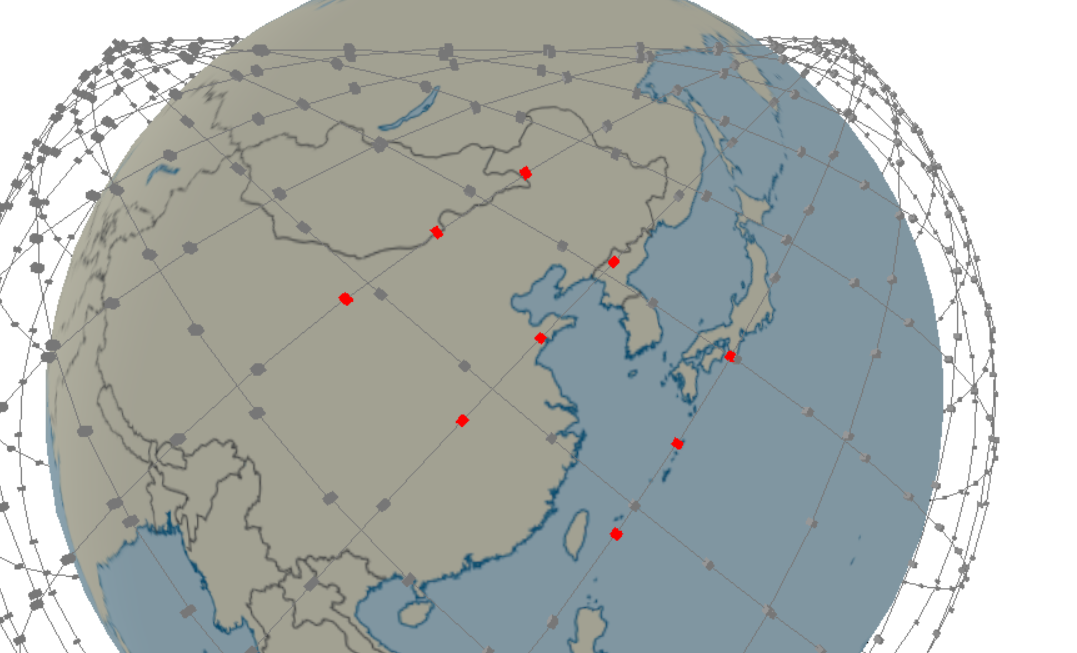
\includegraphics[width=0.5\textwidth]{NearbySats}
\end{SCfigure}

\begin{figure}
\centering
\label{fig:Relative Paths of Satellites}
\caption{An example of the paths that neightbors take relative to a satellite and it's direction of motion.}
\begin{tikzpicture}
\begin{axis}  [xlabel={Distance Perpendicular to Direction Of Motion (km)}, ylabel={Distance in Direction of Motion (km)},width=\textwidth]
\addplot [mark=*, color=black] table [x expr = \thisrow{sat0x} * 1000, y expr = \thisrow{sat0z} * 1000, col sep=comma] {./Data/NearbySats.csv};
\addplot [mark=*, color=red] table [x expr = \thisrow{sat1x} * 1000, y expr = \thisrow{sat1z} * 1000, col sep=comma] {./Data/NearbySats.csv};
\addplot [mark=*, color=orange] table [x expr = \thisrow{sat2x} * 1000, y expr = \thisrow{sat2z} * 1000, col sep=comma] {./Data/NearbySats.csv};
\addplot [mark=*, color=yellow] table [x expr = \thisrow{sat3x} * 1000, y expr = \thisrow{sat3z} * 1000, col sep=comma] {./Data/NearbySats.csv};
\addplot [mark=*, color=green] table [x expr = \thisrow{sat4x} * 1000, y expr = \thisrow{sat4z} * 1000, col sep=comma] {./Data/NearbySats.csv};
\addplot [mark=*, color=blue] table [x expr = \thisrow{sat5x} * 1000, y expr = \thisrow{sat5z} * 1000, col sep=comma] {./Data/NearbySats.csv};
\addplot [mark=*, color=purple] table [x expr = \thisrow{sat6x} * 1000, y expr = \thisrow{sat6z} * 1000, col sep=comma] {./Data/NearbySats.csv};
\addplot [mark=*, color=gray] table [x expr = \thisrow{sat7x} * 1000, y expr = \thisrow{sat7z} * 1000, col sep=comma] {./Data/NearbySats.csv};
\end{axis}
\end{tikzpicture}
\end{figure}

\begin{SCfigure}
\centering
\label{fig:Exchange of Satellites}
\caption{Towards the South Pole, the square of satellites fold over and the satellites that were once on the right of the central satellite move to the left.}
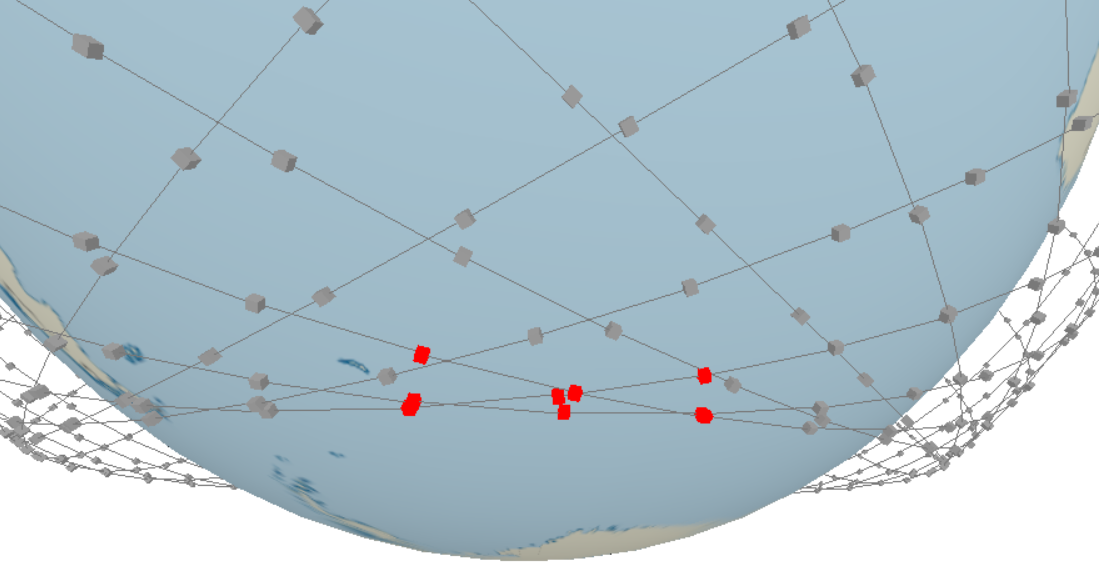
\includegraphics[width=0.5\textwidth]{NearbySats2}
\end{SCfigure}

\begin{figure}
\centering
\label{fig:Sideways Position of Satellites}
\caption{The distance over time from a satellite to it's neighbors perpendicular to it's direction of motion and the direction towards the core of the Earth, or how far to the left or right of the satellite it's neightbors are over time.}
\begin{tikzpicture}
\begin{axis}  [xlabel={Time Passed (minutes)}, ylabel={Distance Perpendicular to Direction of Motion (km)},width=\textwidth]
\addplot [mark=, color=black] table [x=time, y expr = \thisrow{sat0x} * 1000, col sep=comma] {./Data/NearbySats.csv};
\addplot [mark=, color=red] table [x=time, y expr = \thisrow{sat1x} * 1000, col sep=comma] {./Data/NearbySats.csv};
\addplot [mark=, color=orange] table [x=time, y expr = \thisrow{sat2x} * 1000, col sep=comma] {./Data/NearbySats.csv};
\addplot [mark=, color=yellow] table [x=time, y expr = \thisrow{sat3x} * 1000, col sep=comma] {./Data/NearbySats.csv};
\addplot [mark=, color=green] table [x=time, y expr = \thisrow{sat4x} * 1000, col sep=comma] {./Data/NearbySats.csv};
\addplot [mark=, color=blue] table [x=time, y expr = \thisrow{sat5x} * 1000, col sep=comma] {./Data/NearbySats.csv};
\addplot [mark=, color=purple] table [x=time, y expr = \thisrow{sat6x} * 1000, col sep=comma] {./Data/NearbySats.csv};
\addplot [mark=, color=gray] table [x=time, y expr = \thisrow{sat7x} * 1000, col sep=comma] {./Data/NearbySats.csv};
\end{axis}
\end{tikzpicture}
\end{figure}

%-----------------------------------------------------------------------------PERIODICITY IN LATENCIES------------------------------------------------------------------------------------
\subsubsection{Periodicity in Latencies}

When initially examining latencies in the network I noticed a slow transition in the result that appeared to suggest some kind of periodicity. \ref{fig:Latency London To New York} To examine this further, I did a further test, this time running the model for a much longer time. \ref{fig:Latency London To New York Extended} What I found was a periodicity in the latency data of almost exactly one hour. I connected this to the rotation of the earth under the starlink network, which has 24 orbits. To confirm this I ran a third test with the Earth frozen, and found the gradual changes observed initially has disappeared. \ref{fig:Latency London To New York (Not Accounting for Rotation of Earth)} As far as I can tell, this hour-long variation in the latency of a path is not something that Mark Handley accounted for in his research, however to account for it in mine, all latency results for a link will be determined by taking the average of regular samples across an hour of simulated time.

\begin{figure}
\label{fig:Latency London To New York}
\caption{The Latency of the London-New York connection over time}
\begin{tikzpicture}
\begin{axis}  [width=\textwidth, height=\axisdefaultheight,  xlabel={Time (minutes)}, ylabel={RTT (milliseconds)}]
\addplot table [x=Time, y expr=\thisrow{Time of Signal (milliseconds)} * 2, col sep=comma] {./Data/LondonToNewYork.csv};
\end{axis}
\end{tikzpicture}
\end{figure}

\begin{figure}
\label{fig:Latency London To New York Extended}
\caption{The Latency of the London-New York connection over time (extended)}
\begin{tikzpicture}
\begin{axis} [width=\textwidth, height=\axisdefaultheight,  xlabel={Time (minutes)}, ylabel={RTT (milliseconds)}]
\addplot table [x=Time (minutes) ,y expr=\thisrow{Time of Signal (milliseconds)} * 2, col sep=comma] {./Data/LondonToNewYorkAccelerated.csv};
\end{axis}
\end{tikzpicture}
\end{figure}

\begin{figure}
\label{fig:Latency London To New York (Not Accounting for Rotation of Earth)}
\caption{The Latency of the London-New York connection over time when the earth is treates as stationart}
\begin{tikzpicture}
\begin{axis} [width=\textwidth, height=\axisdefaultheight,  xlabel={Time (minutes)}, ylabel={RTT (milliseconds)}] 
\addplot table [x=Time (minutes), y expr=\thisrow{Time of Signal (milliseconds)} * 2, col sep=comma] {./Data/LondonToNewYorkFrozenEarth.csv};
\end{axis}
\end{tikzpicture}
\end{figure}

%==============================================================================================================================
%----------------------------------------------------------------------------------------------------------EVALUATION----------------------------------------------------------------------------------------------------------
%==============================================================================================================================
\section{Evaluation}

My goals going into this project were:

\begin{itemize}
\item To develop multiple routing algorithms for this network.
\item To compare these algorithms on latency, fault tolerance, and response to high demand.
\item To create visualisations of these routing algorithms at work.
\end{itemize}

With success being determined if I can test three different algorithms, producing meaningful data about their latency, fault tolerance, and response under high demand along with informative visualisations of their operations. 

It became apparent early on that "routing algorithms" was a very ambiguous term. It is not clear how one would develop an entirely new routing algorithm to operate on this network, or whether SpaceX would choose to. Furthemore, the behaviour of the network is extremely predictable, which means that a base station can easily calculate the optimal path across the netwrok and send a packet up with the exact satellites it needs to be passed between, this makes static routing the most likely option. What is very much undetermined is the topology of the network being routed across, specifically the linking method and the phase offset. Because of that, I chose to examine the properties of 3 linking methods instead.

%============================================DEVELOPING LINKING METHODS FOR THE NETWORK============================================
\subsection{Developing Linking Methods for the Network}

The three linking methods I chose to examine are

\begin{itemize}
\item
\[\begin{bmatrix} 
1 & 0 \\
0 & 1 
\end{bmatrix} = Handley(0)\]
\item
\[\begin{bmatrix} 
1 & -1 \\
0 & 1 
\end{bmatrix} = Handley(-1)\]
\item
\[\begin{bmatrix} 
2 & 1 \\
-1 & -1 
\end{bmatrix} = DistantLinking\]
\end{itemize}

The first two were variations of the linking methods used by Mark Handley, the third was chosen based off of observations of the network. Specifically I wanted to test whether having satellites "skip" nearby connections for more distant links would lead to an improvement in performance byreducing the number of hops in shortest paths.

%============================================COMPARING LINKING METHODS============================================
\subsection{Comparing Linking Methods}

%-----------------------------------------------------------------------------COMPARING LINKING METHODS ON LATENCY------------------------------------------------------------------------------------
\subsubsection{Comparing Linking Methods On Latency}

%-----------------------------------------------------------------------------COMPARING LINKING METHODS ON FAULT TOLERANCE------------------------------------------------------------------------------------
\subsubsection{Comparing Linking Methods On Fault Tolerance}

The first test I did for fault tolerance was a simple test of total connectivity. I deleted a certain percentage of satellites from each linking method, and then tested the total number of connected components. I did this 100 times, so that my 95\% confidence interval never exceeded 4 components. What I found is that all 3 linking methods had exactly the same curve of connected components, with the expected umber of connected components rising after a 20\% faliure rate, peaking at an 80\% faliure rate, and than dropping off as the number of satellites being removed from the constellation outpaced the number of tnew constellations being crates.

\begin{figure}
\label{fig:Connected Components After Deletions}
\caption{The number of connected components after various amounts of deletion of random satellites, using the three linking methods outlined.}
\begin{tikzpicture}
\begin{axis}  [ xlabel={Proportion of Satellites Failed}, ylabel={Average Number of Connected Components}, legend pos = north west]
\addplot +[mark=, error bars/.cd, y dir = both, y explicit] table [x=FaliureRate, y=ConnectedComponents, col sep=comma, y error = Error] {./Data/ConnectedComponentsLM1 - Results.csv};
\addlegendentry{Handley(-1)}
\addplot +[mark=, error bars/.cd, y dir = both, y explicit] table [x=FaliureRate, y=ConnectedComponents, col sep=comma, y error = Error] {./Data/ConnectedComponentsLM2 - Results.csv};
\addlegendentry{Handley(0)}
\addplot +[mark=, error bars/.cd, y dir = both, y explicit] table [x=FaliureRate, y=ConnectedComponents, col sep=comma, y error = Error] {./Data/ConnectedComponentsLM3 - Results.csv};
\addlegendentry{DistantLinking}
\end{axis}
\end{tikzpicture}
\end{figure}

%-----------------------------------------------------------------------------COMPARING LINKING METHODS ON RESPONSE TO HIGH DEMAND------------------------------------------------------------------------------------
\subsubsection{Comparing Linking Methods On High Demand}

%============================================VISUALISING THE LINKING METHODS AT WORK============================================

\subsection{Visualising the Linking Methods at Work}

















%++++++++++++++++++++++++++++++++++++++++++++++++++++++++++++++++++++++++++++++++++++++++++++++++++++++++++++++++++++++++++++++++++++++++++++++++++++++++++++++++++++++++++++++++++++++++++++++++++++++++

%\begin{figure}
%\label{fig:Latency London To New York (Smoothed)}
%\caption{The Average Latency of the London-New York connection over time}
%\begin{tikzpicture}
%\begin{axis} [width=\textwidth, height=\axisdefaultheight] 
%\addplot table [x=Time (minutes), y=Latency (smooth), col sep=comma] {./Data/LondonToNewYorkAcceleratedSmooth.csv};
%\end{axis}
%\end{tikzpicture}
%\end{figure}


%TODO FIGURE OF LONG PATH
%DISTANCE 130
%990 Sats in constellation

%From observations of the simulations, when there were faliures in the network, it was almost always caused by a base station not having any satellites overhead to connect with. Near the equator, a base station may only have one or two satellites directly 

\subsection{Direction and Focus}

Maintaining a consistent goal has been challenging during such an open-ended project. If I were to do this project again I would more carefully choose my orbjectives %TODO

A number of projects in the early phrases of the project had to be abandoned not just because of inefficenfiency but because new information came about that rendered hem useless.

The announcement from SpaceX on that they were significantly changing the constellation had massive impacts to the project. Firstly, the new satellites would have only four links instead of five, this implied that the satellites would not not have a "free" link but would instead be connected only to those ahead of and behind them. Because of this, I decided to drop the free links from my model, but doing so meant that a large chunk of code that had been written was discarded.

The knowledge that SpaceX were willing to change their designs so abruptly also had a sigificant impact on modelling their constellation. It is likely that the second and third phases of Starlink will be similarly changed to be in similar altitudes to phase one, however without a full understanding on what these new spheres would be, or how they would connect to phase one, it was elected to instead focus slely on the first sphere's constellation. %Detail announcement

\subsection{Extension}

In Handley's original paper, he anticipated ...

%==============================================================================================================================
%----------------------------------------------------------------------------------------------------------CONCLUSION---------------------------------------------------------------------------------------------------------
%==============================================================================================================================
\section{Conclusion}

I beleive that I have made a number of very significant extensions to Handley's work. The discovery of the 60-minute variations in latencies is in my opinion very significant, this is something that I have not seen observed in any of the research thusfar but has a significant impact on how one calculates latencies across the netork.

%TODO

\begin{thebibliography}{99}
	%using the vancouver system https://en.wikipedia.org/wiki/Vancouver_system
	\bibitem{ExedeWebsite} \url{https://www.exede.com}
	\bibitem{HughesWebsite} \url{https://www.hughes.com}
	\bibitem{ElonMuskTweet} \url{https://twitter.com/elonmusk/status/1000453321121923072}
	\bibitem{FCCApplication} \url{licensing.fcc.gov/cgi-bin/ws.exe/prod/ib/forms/reports/related_filing.hts?f_key=-289550&f_number=SATLOA2016111500118}
	\bibitem{TechnicalAttachment} \url{https://licensing.fcc.gov/myibfs/download.do?attachment_key=1158350}
	\bibitem{OriginalReport} \url{http://nrg.cs.ucl.ac.uk/mjh/starlink/}
	\bibitem{StuffInSpace} \url{http://stuffin.space/}
	\bibitem{PropertiesOfGlass} \url{http://ece466.groups.et.byu.net/notes/smf28.pdf}
	\bibitem{HughesPressRelease} \url{https://www.hughes.com/who-we-are/resources/press-releases/hughes-high-throughput-satellite-successfully-launched-setting?locale=en}
	\bibitem{EchoStar} \url{https://space.skyrocket.de/doc_sdat/jupiter-2.htm}
	\bibitem{KABand} \url{file:///home/joe/Downloads/R12-ITURKA.BAND-C-0008!!PDF-E.pdf}
	\bibitem{FirstPersonMotion} \url{https://github.com/turtletooth/GodotFirstPersonController}
	\bibitem{Map} \url{https://commons.wikimedia.org/wiki/File:USGS_majplatecolor.png}
\end{thebibliography}
\appendix

\section{Appendix A}

\printindex

%TODO Project Proposal

\end{document}